% Compile with:
% latexmk -pvc -interaction=nonstopmode *Seminar.tex
\documentclass[aspectratio=169,10pt]{beamer}
%\documentclass[aspectratio=169,10pt,draft]{beamer}
\usetheme[language=english]{ubbeamer2023}

\title{Tomographic imaging of fish}
\subtitle{Or how to image, \emph{many} more teeth}
\author{David Haberthür}
\institute{Institute of Anatomy}
\date{September 19, 2024}

% Some often used abbreviations/commands
\newcommand{\everyframe}{2}% use only every nth frame for the animations
\newcommand{\imagewidth}{\columnwidth}% set global image width
\newcommand{\imageheight}{0.7\paperheight}% set global image height
\newlength\imagescale% needed for scalebars
\newcommand{\uct}{{\textmu}CT\xspace}% make our life easier
\newcommand{\eg}{e.\,g.\xspace}%
\newcommand{\ie}{i.\,e.\xspace}%

\usepackage[%
	backend=biber,%
	sorting=none,%
	style=ieee,% `ieee` is needed for hypercite/footcite at the bottom of the slides
	citetracker=true,%
	isbn=false,%
	url=false,%
	maxnames=1,minnames=1,% Show only first author in references
	]{biblatex}%
% Globally remove stuff from bibliography
% https://tex.stackexchange.com/a/25232
\DeclareSourcemap{%
  \maps[datatype=bibtex]{%
    \map{%
      \step[fieldset=journal, null]%
      \step[fieldset=editor, null]%
      \step[fieldset=volume, null]%
      \step[fieldset=number, null]%
      \step[fieldset=pages, null]%
      \step[fieldset=year, null]%
    }%
  }%
}%
% Fix double-comma in footcite
% Copy the relevant line from https://tex.stackexchange.com/a/409861/828
\renewcommand\labelnamepunct{\adddot\space} %punct after autor
\addbibresource{../../Documents/library.bib}% FastSSD, Windows or Mac works (on Linux/FastSSD we generated a 'Document' folder at the correct level and `ln -s ~/P/Documents/library.bib .` to it)
\usepackage{tikz}
	\usetikzlibrary{shadows,spy}
	\tikzset{shadowed/.style={preaction={transform canvas={shift={(1pt,-1pt)}},draw=ubRed}}}
\usepackage{shadowtext}
	\shadowoffset{1pt}
	\shadowcolor{ubRed}
\usepackage{microtype}
\usepackage[detect-all=true,
	range-phrase=--,
	range-units=single,
	per-mode=symbol,
	per-symbol=/]{siunitx}
\usepackage{animate}	
\usepackage{gitinfo2}
\usepackage{xspace}
\usepackage{fontawesome5}
\usepackage{csquotes}
\usepackage{listings}
	\lstset{basicstyle=\scriptsize\ttfamily}

% Globally thicker lines in with tikz
% https://tex.stackexchange.com/a/206769/828
\tikzset{every picture/.style={thick}}

% Globally set up scale bar, drawn with https://github.com/habi/latex/blob/master/draw_a_scalebar.py
\tikzset{shadowed/.style={preaction={transform canvas={shift={(1pt,-1pt)}},draw=ubRed}}} % shadowed drawing https://tex.stackexchange.com/a/185853/828
\pgfmathsetlength{\imagewidth}{\imagewidth}%

% Acknowledge images just below them
% Based on https://tex.stackexchange.com/a/282637/828
\newcommand{\source}[2]{%
	% Print out (short) link under image, with small text
	\raisebox{-1.618ex}{%
		\makebox[0pt][r]{%
			\tiny\href{http://#1}{#1} #2%
			}%
		}%
	}%
\newcommand{\sourcecite}[2]{%
	% Cite (an image from) a reference
	\raisebox{-1.618ex}{%
		\makebox[0pt][r]{%
			\tiny From~\cite{#1}, #2%
			}%
		}%
	}%
\newcommand{\sourcelink}[3]{%
	% Make the source command an \href{link}{text}
	\raisebox{-1.618ex}{%
		\makebox[0pt][r]{%
			\tiny\href{#1}{#2}, #3%
			}%
		}%
	}%

% Make us a nice citation command for citing in a footnote
% https://tex.stackexchange.com/a/396754/828
\makeatletter
\newbibmacro*{hypercite}{%
	\renewcommand{\@makefntext}[1]{\noindent\normalfont##1}%
	\footnotetext{%
		\blxmkbibnote{foot}{%
			\printtext[labelnumberwidth]{%
				\printfield{prefixnumber}%
				\printfield{labelnumber}%
			}%
			\addspace%
			\fullcite{\thefield{entrykey}}%
			}%
		}%
	}%
\DeclareCiteCommand{\hypercite}%
	{\usebibmacro{cite:init}}%
	{\usebibmacro{hypercite}}%
	{}%
	{\usebibmacro{cite:dump}}%
% Redefine the \footcite command to use the reference number
\renewcommand{\footcite}[1]{\cite{#1}\hypercite{#1}}
\makeatother
% Remove title when using footcite/hypercite
\AtEveryCitekey{\clearfield{title}}

\begin{document}
\begin{frame}
	\maketitle
\end{frame}

 \begin{frame}
 	\frametitle{Grüessech mitenang!}
 	\begin{itemize}
 		\item David Haberthür
 		\begin{itemize}
 			\item Physicist by trade
 			\item \href{https://boris.unibe.ch/2619/}{PhD in high resolution imaging of the lung}, Institute of Anatomy, University of Bern, Switzerland
 			\item Post-Doc I: \href{https://www.psi.ch/sls/tomcat/}{TOMCAT}, \href{https://www.psi.ch/sls/}{Swiss Light Source}, \href{https://www.psi.ch/}{Paul Scherrer Institute}, Switzerland
 			\item Post-Doc II/Technisch-wissenschaftliche Arbeit 1: \uct group, Institute of Anatomy, University of Bern, Switzerland.
 		\end{itemize}
 	\end{itemize}
 \end{frame}

 \begin{frame}
 	\frametitle{MicroCT group}
 	\centering%
 	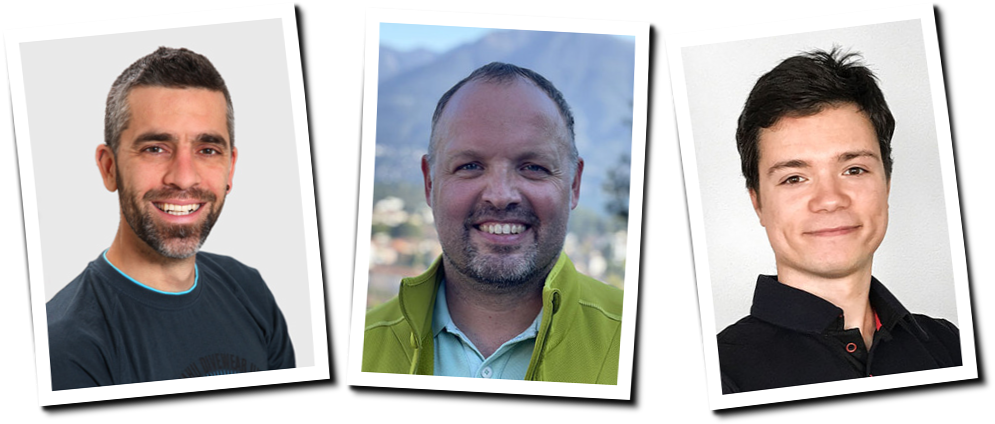
\includegraphics[width=\imagewidth]{./media/team}%
 	\hfill%
 	David{\color{ubRed}.}Haberthuer{\color{ubRed}@unibe.ch}%
 	\hfill%
 	Ruslan{\color{ubRed}.}Hlushchuk{\color{ubRed}@unibe.ch}%
 	\hfill%
 	Oleksiy{\color{ubRed}.}Khoma{\color{ubRed}@unibe.ch}%
 	\hfill%
 \end{frame}

\begin{frame}
 	\frametitle{MicroCT group}
	\begin{columns}
		\begin{column}{0.5\linewidth}
 			\begin{itemize}
 				\item microangioCT~\cite{Hlushchuk2018}
 				\begin{itemize}
 					\item Angiogenesis: heart, musculature~\cite{Nording2021} and bones
 					\item Vasculature: (mouse) brain~\cite{Hlushchuk2020}, (human) nerve scaffolds~\cite{Wuthrich2020}, (human) skin flaps~\cite{Zubler2021} and tumors
 				\end{itemize}
 				\item Zebrafish musculature and gills~\cite{MesserliAaldijk2020}
 				\item (Lung) tumor detection and metastasis classification~\cite{Trappetti2021}
 				\item Collaborations with museums~\cite{Bochud2021} and scientist at UniBe~\cite{Halm2021,Kadlag2023} to scan a wide range of specimens, from human hearing bones to meteorites
 				\item Automate \emph{all} the things!~\cite{Haberthuer2021,Haberthuer2023}
 			\end{itemize}
		\end{column}
		\begin{column}{0.5\linewidth}
 			\vfill%
 			\includegraphics<1>[width=\imagewidth]{./media/1172}%
 			\only<1>{\source{brukersupport.com}{}}%
 			\vfill%
 			\includegraphics<2>[width=\imagewidth]{./media/1272}%
 			\only<2>{\source{bruker.com/skyscan1272}{}}%
 			\vfill%
 			\includegraphics<3>[width=\imagewidth]{./media/2214}%
 			\only<3>{\source{bruker.com/skyscan2214}{}}%
 			\vfill%
		\end{column}
	\end{columns}
\end{frame}

\begin{frame}
	\frametitle{What about those teeth?}
	\begin{columns}
		\begin{column}{0.5\linewidth}		
			Collaboration with \href{https://www.zmk.unibe.ch/}{zmk bern – Zahnmedizinische Kliniken}~\footcite{Haberthuer2021,Wolf2021}
			\begin{itemize}
				\item 104 extracted human permanent mandibular canines
				\item Segmentation of teeth and root canal
				\item Numbers instead of just pretty images, unbiased characterization
				\item Reproducible and automated image analysis with \href{https://www.python.org/}{\faPython} in \href{https://jupyter.org/}{Jupyter}~\cite{Kluyver2016}
			\end{itemize}
		\end{column}
		\begin{column}{0.5\linewidth}
			\centering%
			\renewcommand{\imagewidth}{0.7\linewidth}
			\only<1>{%
				\pgfmathsetlength{\imagescale}{\imagewidth/2716}%
				\def\x{1678}% scalebar-x starting at golden ratio of image width of 2716px = 1678
				\def\y{2444}% scalebar-y at 90% of image height of 2716px = 2444
				\begin{tikzpicture}[x=\imagescale,y=-\imagescale]
					\node[anchor=north west, inner sep=0pt, outer sep=0pt] at (0,0) {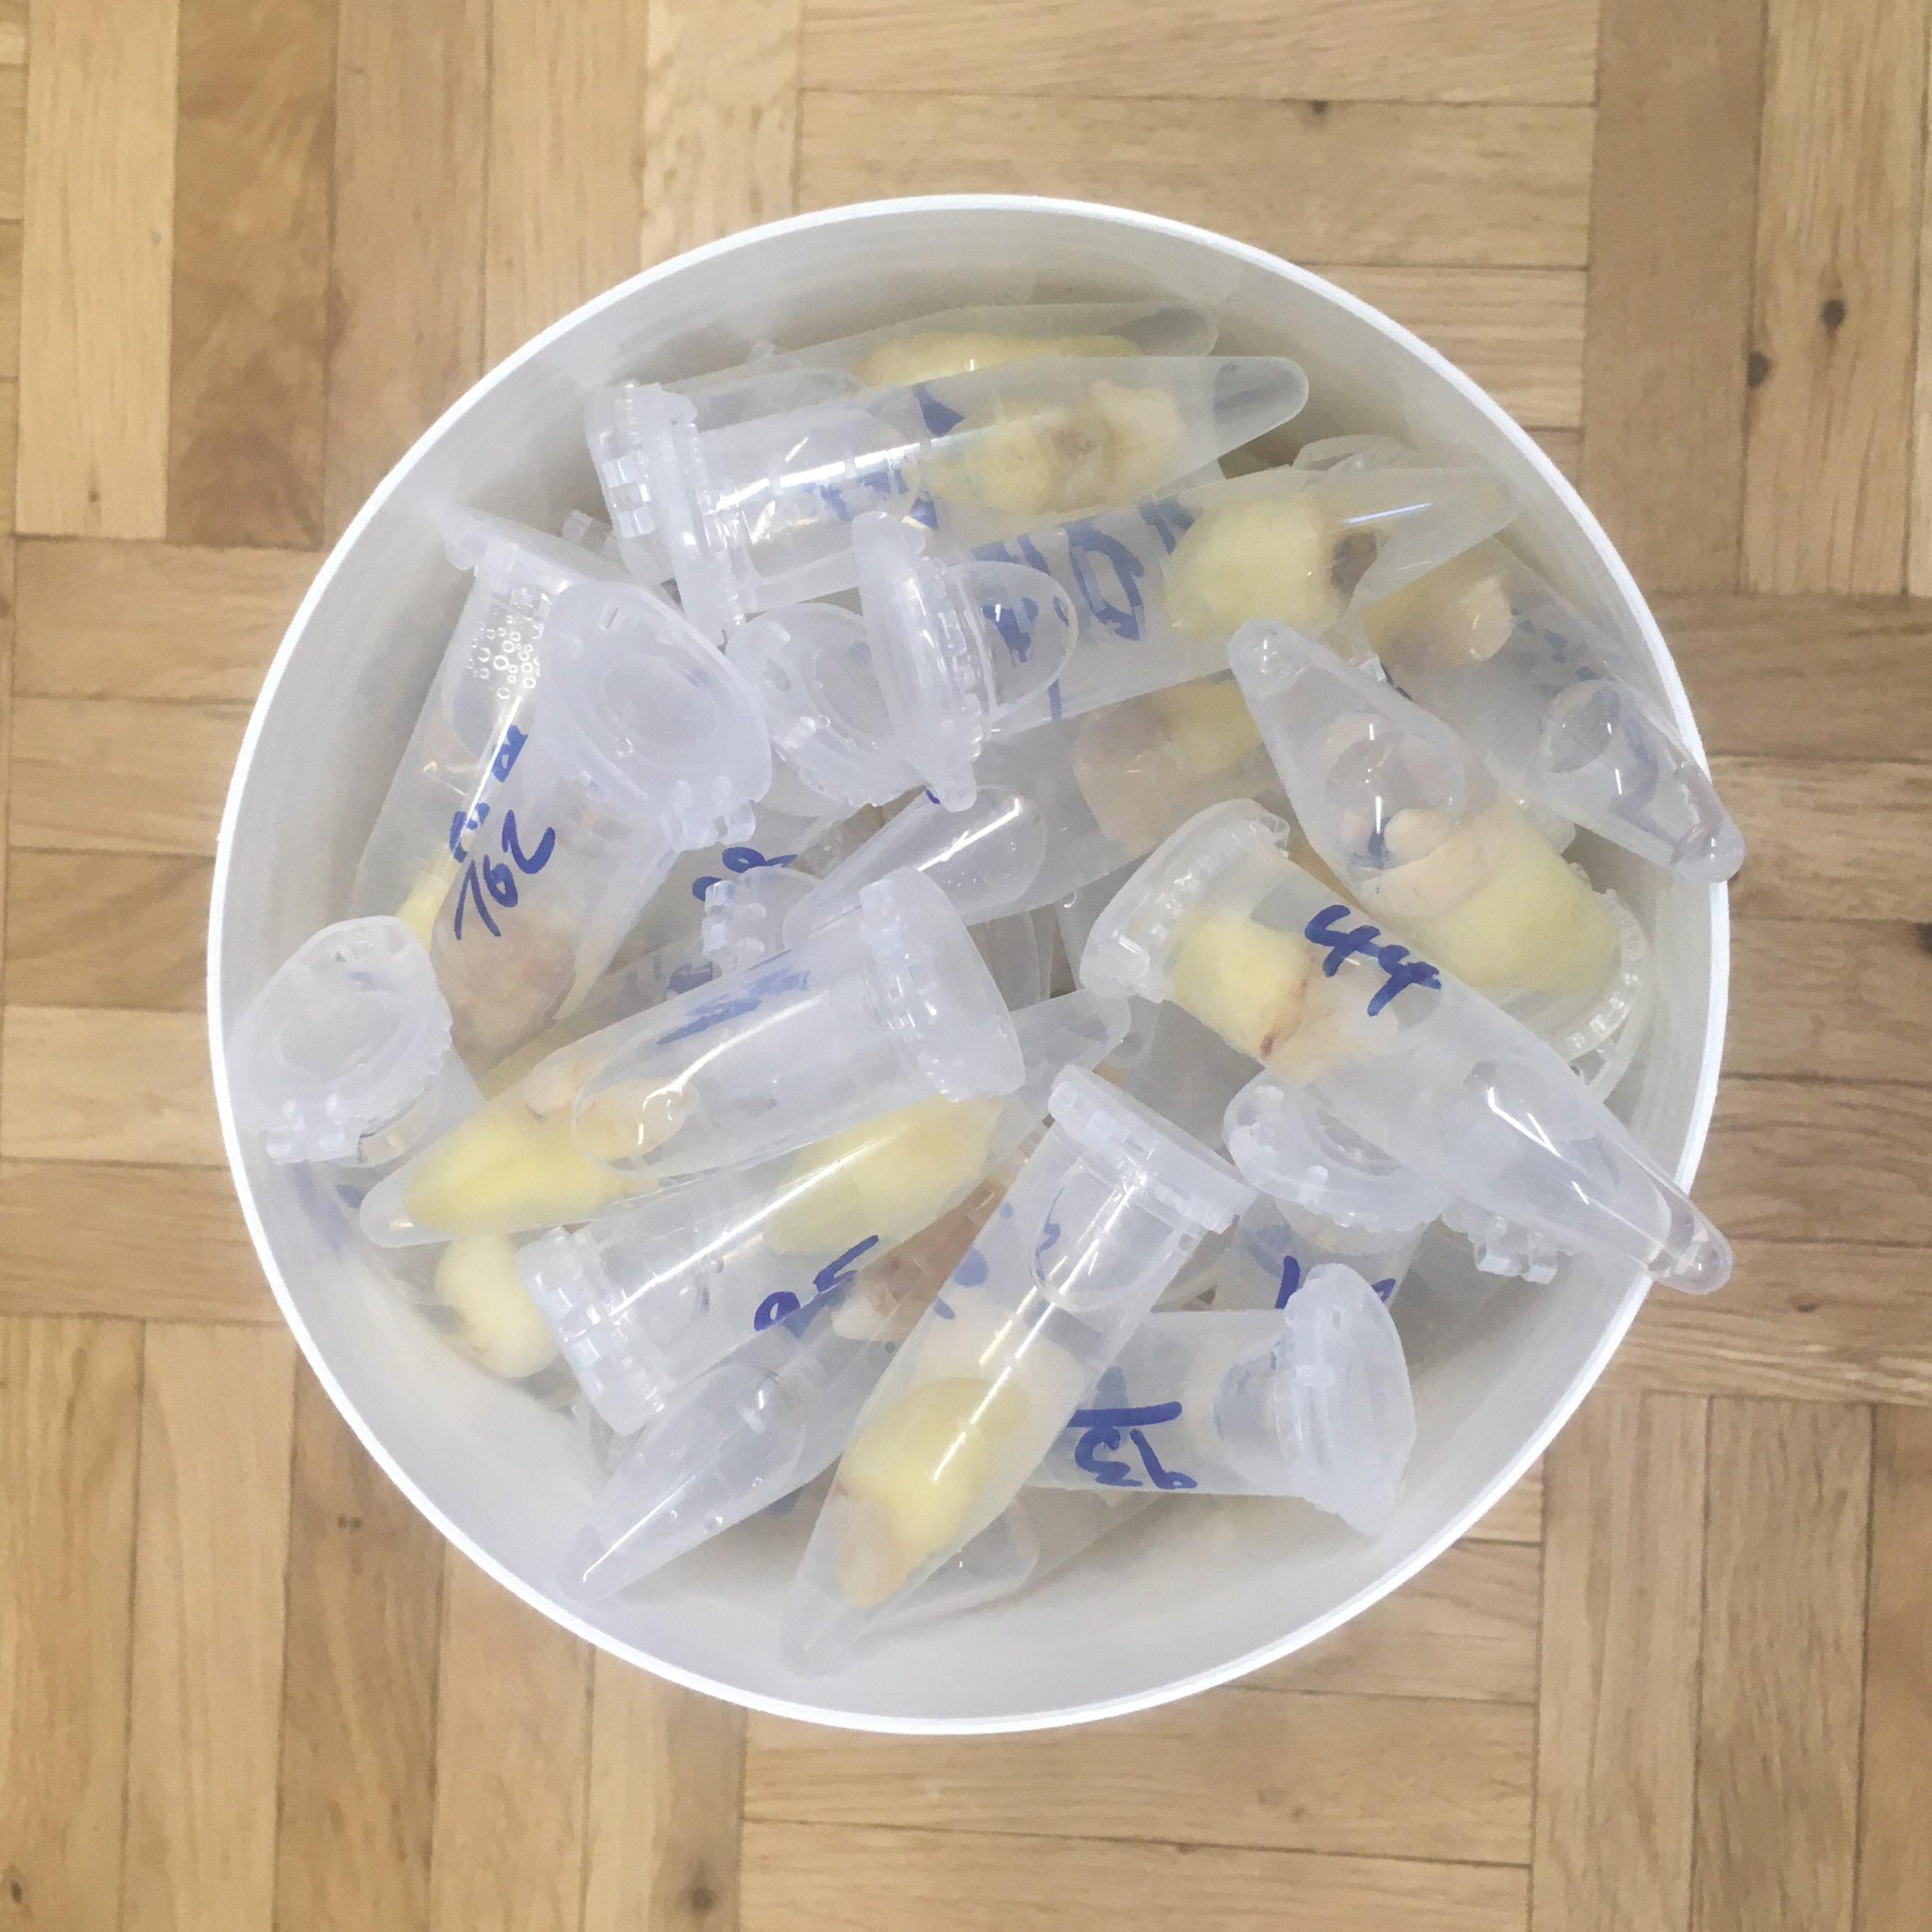
\includegraphics[width=\imagewidth]{./media/bucketofteeth}};
					% 2132.087px = 140.0mm -> 100px = 6566.337um -> 7.615px = 500um, 1.523px = 100um
					%\draw[|-|,blue,thick] (299,1340) -- (2430,1406) node [sloped,midway,above,fill=white,semitransparent,text opacity=1] {\SI{140.0}{\milli\meter} (2132px) TEMPORARY!};
					\draw[|-|,white,thick,shadowed] (\x,\y) -- (\x+761.5,\y) node [midway,above] {\shadowtext{\SI{5}{\centi\meter}}};
				\end{tikzpicture}%
				}%
			\renewcommand{\imagewidth}{\columnwidth}
 	 		\begin{tikzpicture}[remember picture,overlay]%		  
 				\only<2>{%
 					\node at (current page.center) [shift={(0,-2.9mm)}]{% 2.9mm comes from the unibe template
						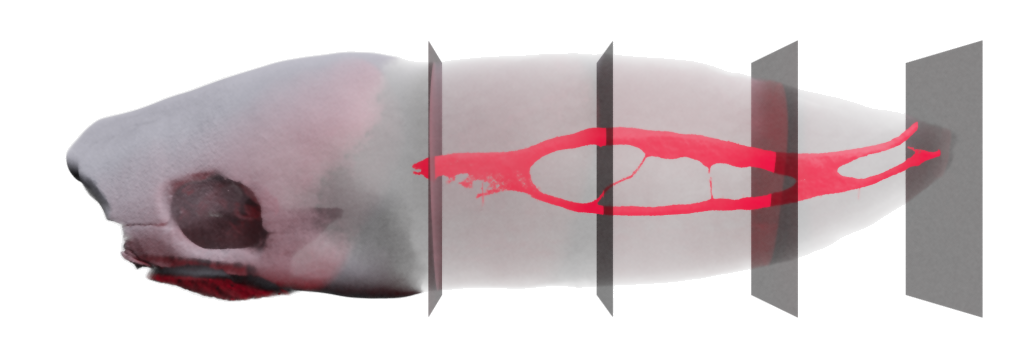
\includegraphics[width=\paperwidth]{./media/ZMK/tooth045/transparent-slices-rcs/image0000}};%
 					}%
 				% Sticky note overlay from https://tex.stackexchange.com/a/159690/828
				% To show it on both slides, we need to put it in the tikzpicture and `only<2>' the teeth
				\node at (current page.center) [shift={(0,-2.9mm)},drop shadow={shadow xshift=2pt,shadow yshift=-4pt}, inner xsep=7pt, fill=yellow, xslant=-0.25, yslant=0.25, inner ysep=10pt] {\parbox[t]{3.5cm}{\emph{How to study the internals of +100 human teeth with X-ray microtomography}\\\\ November 12, 2020}};%
			\end{tikzpicture}%
		\end{column}%	
	\end{columns}
\end{frame}

\begin{frame}
	\frametitle{Many more teeth, but from Cichlids}
			\begin{columns}
			\begin{column}{0.5\linewidth}
		 	Collaboration with team of \href{https://www.aqua.iee.unibe.ch/}{\emph{Aquatic Ecology \& Evolution}}, from the \href{https://www.iee.unibe.ch/}{Institute of Ecology and Evolution}~\footcite{Haberthuer2023}
		\begin{itemize}
 		 		 	\item 133 Cichlids from Lake Victoria, East Africa
					\begin{itemize}
						\item Functional anatomy of the skulls and jaws
						\item<2-> \qtyrange{6}{18}{\centi\meter} in size
					\end{itemize}
					\item<7-> 375 scans in total
		 			\begin{itemize}
						\item<7-> Voxelsizes from \qtyrange{3.5}{50}{\micro\meter}
		 				\item<7-> 46 days of scanning time
		 				\item<7-> \qty{9.8}{\tera\byte} of raw data
		 				\item<7-> \qty{1.5}{\tera\byte}/+\num{1000000} reconstructions
		 			\end{itemize}
		 		\end{itemize}
			\end{column}
			\begin{column}{0.5\linewidth}
				\centering
				\only<1>{%
					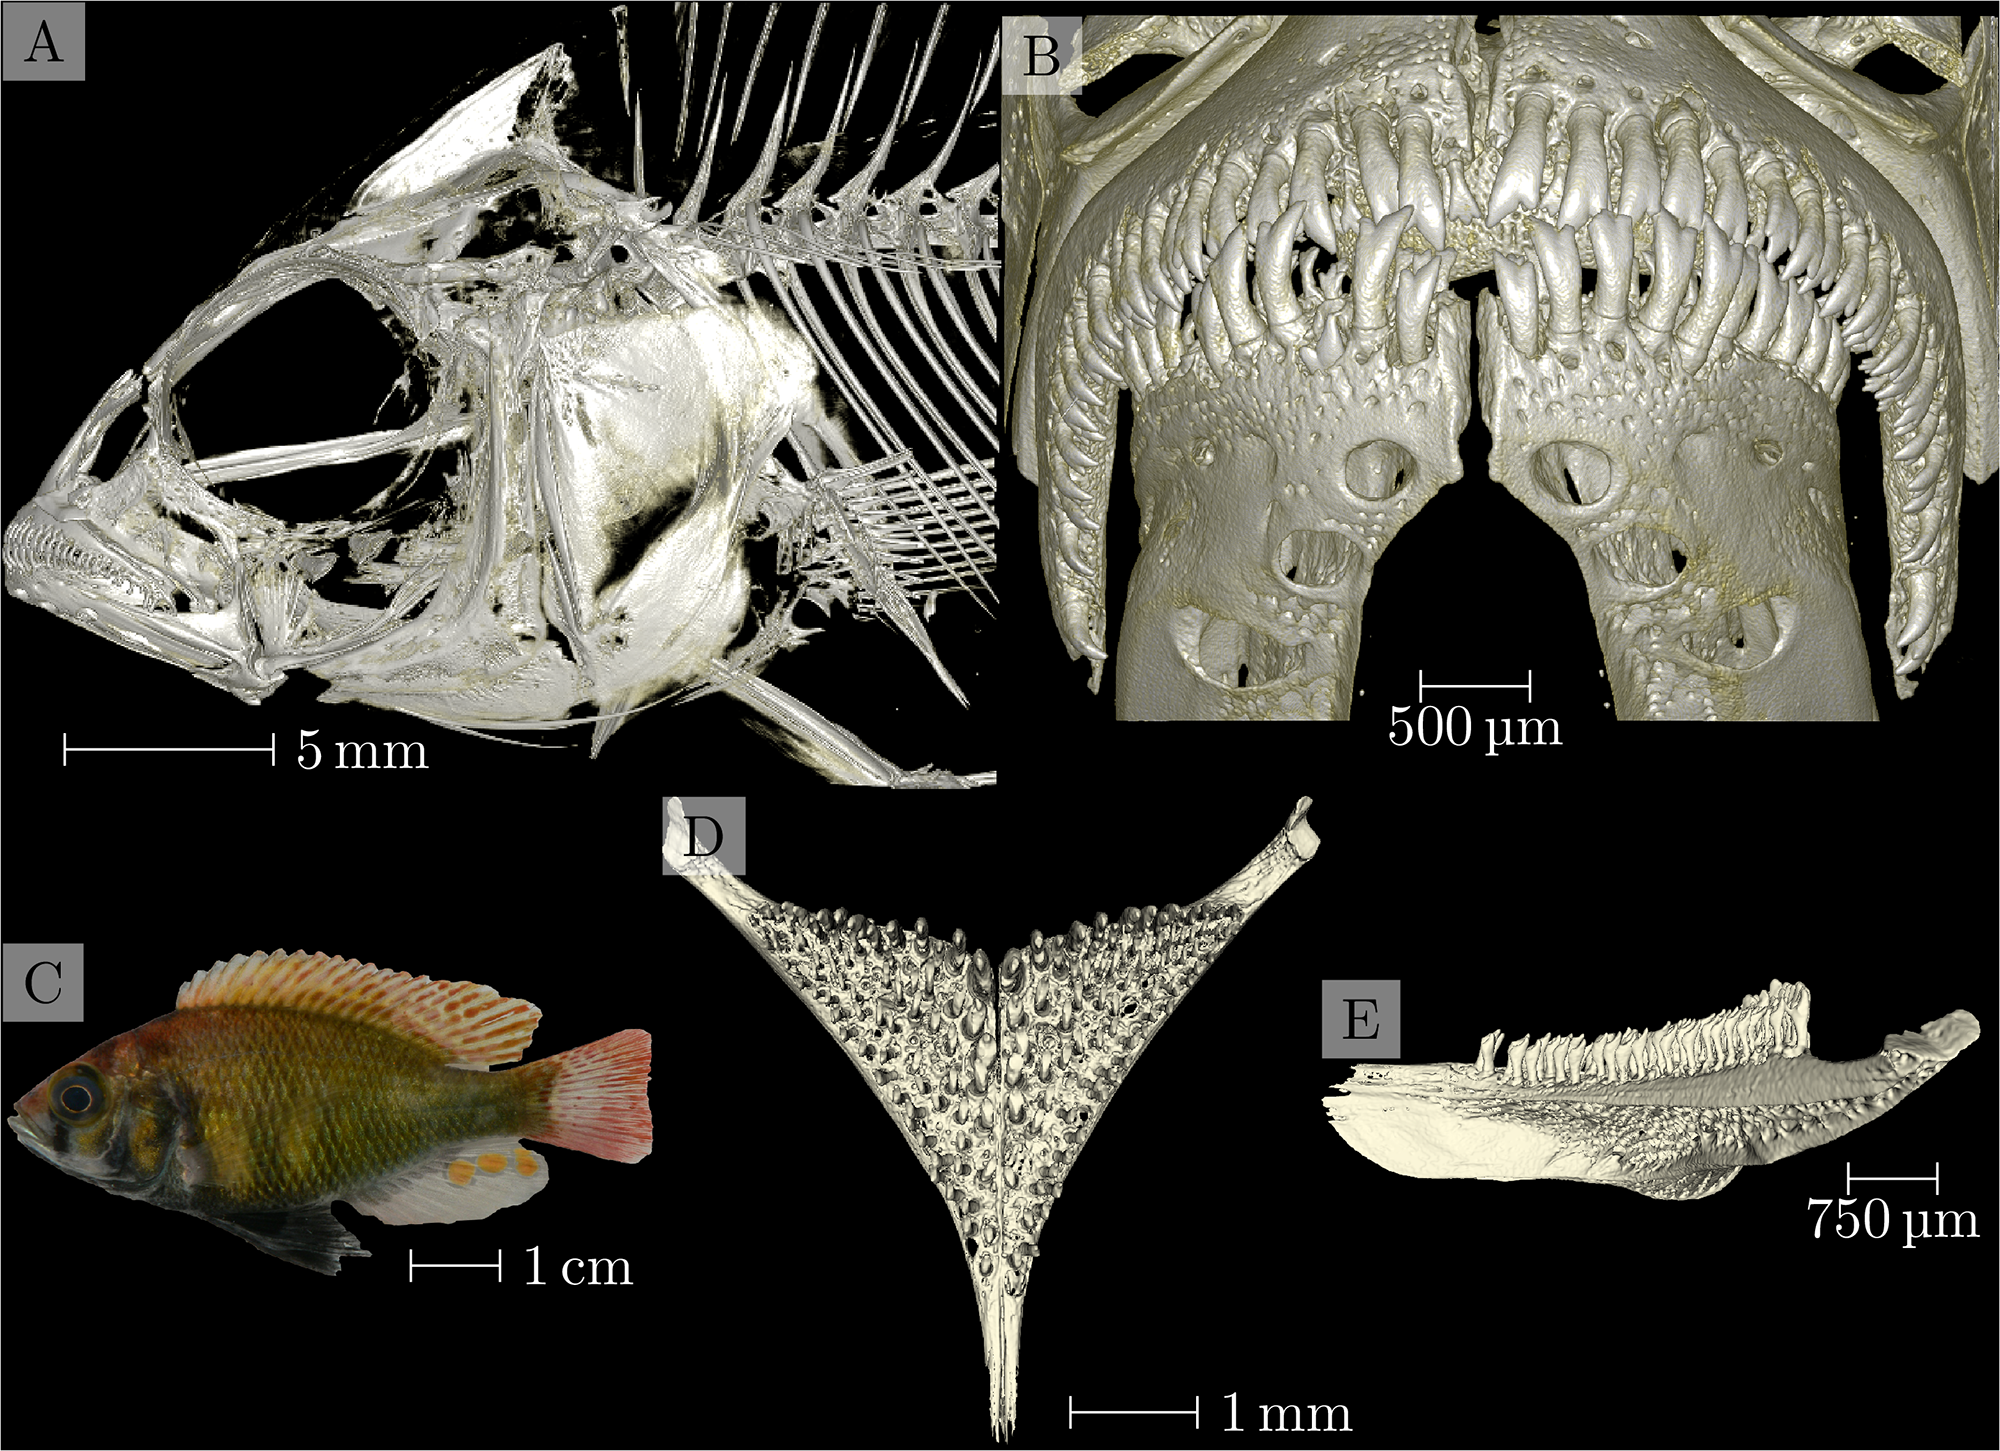
\includegraphics[width=\imagewidth]{./media/EAWAG/journal.pone.0291003.g001.png}%
					\sourcelink{https://doi.org/10.1371/journal.pone.0291003.g001}{DOI:gsst8t}{Fig.~1}%
					}%
				\includegraphics<2>[width=\imagewidth]{./media/EAWAG/lengths.plot.png}%
				\includegraphics<3>[width=\imagewidth]{./media/EAWAG/lengths.violinplot.png}%
				\includegraphics<4>[width=\imagewidth]{./media/EAWAG/lengths.boxplot.png}%
				\includegraphics<5>[width=\imagewidth]{./media/EAWAG/lengths.boxenplot.png}%
				\includegraphics<6>[width=\imagewidth]{./media/EAWAG/lengths.boxenplot.only.png}%
				\includegraphics<7>[width=\imagewidth]{./media/EAWAG/voxelsizes.png}%
			\end{column}
		\end{columns}
\end{frame}

\begin{frame}
	\frametitle{Visualization of cichlid head}
	\centering%
	% Generate animations in ImageJ with 3Dscript (files are in repository)
	% Save out as .tif slices
	% mogrify -format png -transparent "rgb(255,255,255)" -fuzz 4% *.tif
	\only<1>{%
		% Show PJ
		\begin{tikzpicture}[remember picture,overlay]%
			\node at (current page.center) {%
				\animategraphics[autoplay,width=\paperwidth,every=\everyframe]{24}{./media/EAWAG/animation.head/104016.head.rec.animation.0}{000}{480}%
			};%
		\end{tikzpicture}%
	}%
	\only<2>{%
		% Show Otolith
		\begin{tikzpicture}[remember picture,overlay]%
			\node at (current page.center) {%
			\animategraphics[autoplay,width=\paperwidth,every=\everyframe]{24}{./media/EAWAG/animation.head/104016.head.rec.animation.}{0481}{1680}%
			};%
		\end{tikzpicture}%			
	}%
	\only<3>{%
		%Move to PJ
		\begin{tikzpicture}[remember picture,overlay]%
			\node at (current page.center) {%
			\animategraphics[autoplay,width=\paperwidth,every=\everyframe]{24}{./media/EAWAG/animation.head/104016.head.rec.animation.}{1681}{1920}%
			};%
		\end{tikzpicture}%
	}%
\note{Fish 104016, Scan head_rec; This fish was scanned on 2022-01-27T13:32:59 on the SkyScan2214, with a voxel size of 13.0 μm.}
\end{frame}

\begin{frame}
	\frametitle{Visualization of segmented pharyngeal jaw}
	\centering
	\only<1>{%
		%Animate from head-dataset to segmented pj
		\begin{tikzpicture}[remember picture,overlay]%
			\node at (current page.center) {%
			\animategraphics[autoplay,width=\paperwidth,every=\everyframe]{24}{./media/EAWAG/animation.head2pj/morphed.0}{000}{240}%
			};%
		\end{tikzpicture}
		}%
	\only<2>{%
		\begin{tikzpicture}[remember picture,overlay]%
			\node at (current page.center) {%
				\animategraphics[autoplay,width=\paperwidth,every=\everyframe]{24}{./media/EAWAG/animation.pj/104016.pj.animation.0}{000}{700}%
			};%
		\end{tikzpicture}%	
	}%
	\only<3>{%
	\begin{tikzpicture}[remember picture,overlay]%
		\node at (current page.center) {%
			\animategraphics[autoplay,width=\paperwidth,every=\everyframe]{24}{./media/EAWAG/animation.pj/104016.pj.animation.}{0701}{1440}%
		};%
	\end{tikzpicture}%	
}%	
\note{Fish 104016, Scan pharynx_rec; This fish was scanned on 2021-02-04T13:30:11 on the SkyScan1272, with a voxel size of 5.0 μm.}
\note{A human hair typically has a thickness ranging from 17 to 181 micrometers (microns), depending on various factors like the individual's hair type, age, and ethnicity. On average, most human hair strands fall between 50 to 100 micrometers in diameter.}
\end{frame}

\begin{frame}
	\frametitle{Data wrangling by example: Cichlids}
	\centering%
	\includegraphics<1>[width=\imagewidth]{./media/EAWAG/Otolither_104016_head_01_Overview}%
	\includegraphics<2>[width=\imagewidth]{./media/EAWAG/Otolither_104016_head_02_GrayValues}%
	\includegraphics<3>[width=\imagewidth]{./media/EAWAG/Otolither_104016_head_03_GrayValuesRegion}%
	\includegraphics<4>[width=\imagewidth]{./media/EAWAG/Otolither_104016_head_04_GrayValuesSmoothed}%
	\includegraphics<5>[width=\imagewidth]{./media/EAWAG/Otolither_104016_head_05_Peaks}%
	\includegraphics<6>[width=\imagewidth]{./media/EAWAG/Otolither_104016_head_06_Peaks_All}%
	\includegraphics<7>[width=\imagewidth]{./media/EAWAG/Otolither_104016_head_07_ExtractedRegions}%
	\includegraphics<8>[width=\imagewidth]{./media/EAWAG/Otolither_104016_head_08_ExtractedRegionsMIPs}%
	\includegraphics<9>[width=\imagewidth]{./media/EAWAG/Otolither_104016_head_09_ExtractedOtolithMasked}%
	\only<10>{\href{https://htmlpreview.github.io/?https://github.com/habi/EAWAG-manuscript/blob/main/content/data/104016_Enterochromis_I_cinctus_St_E.head.rec.Otolith.Region.3D.html}{Exported 3D view}}%
\end{frame}

\begin{frame}
	\frametitle{What to do now?}
	\centering%
	\only<1>{%
		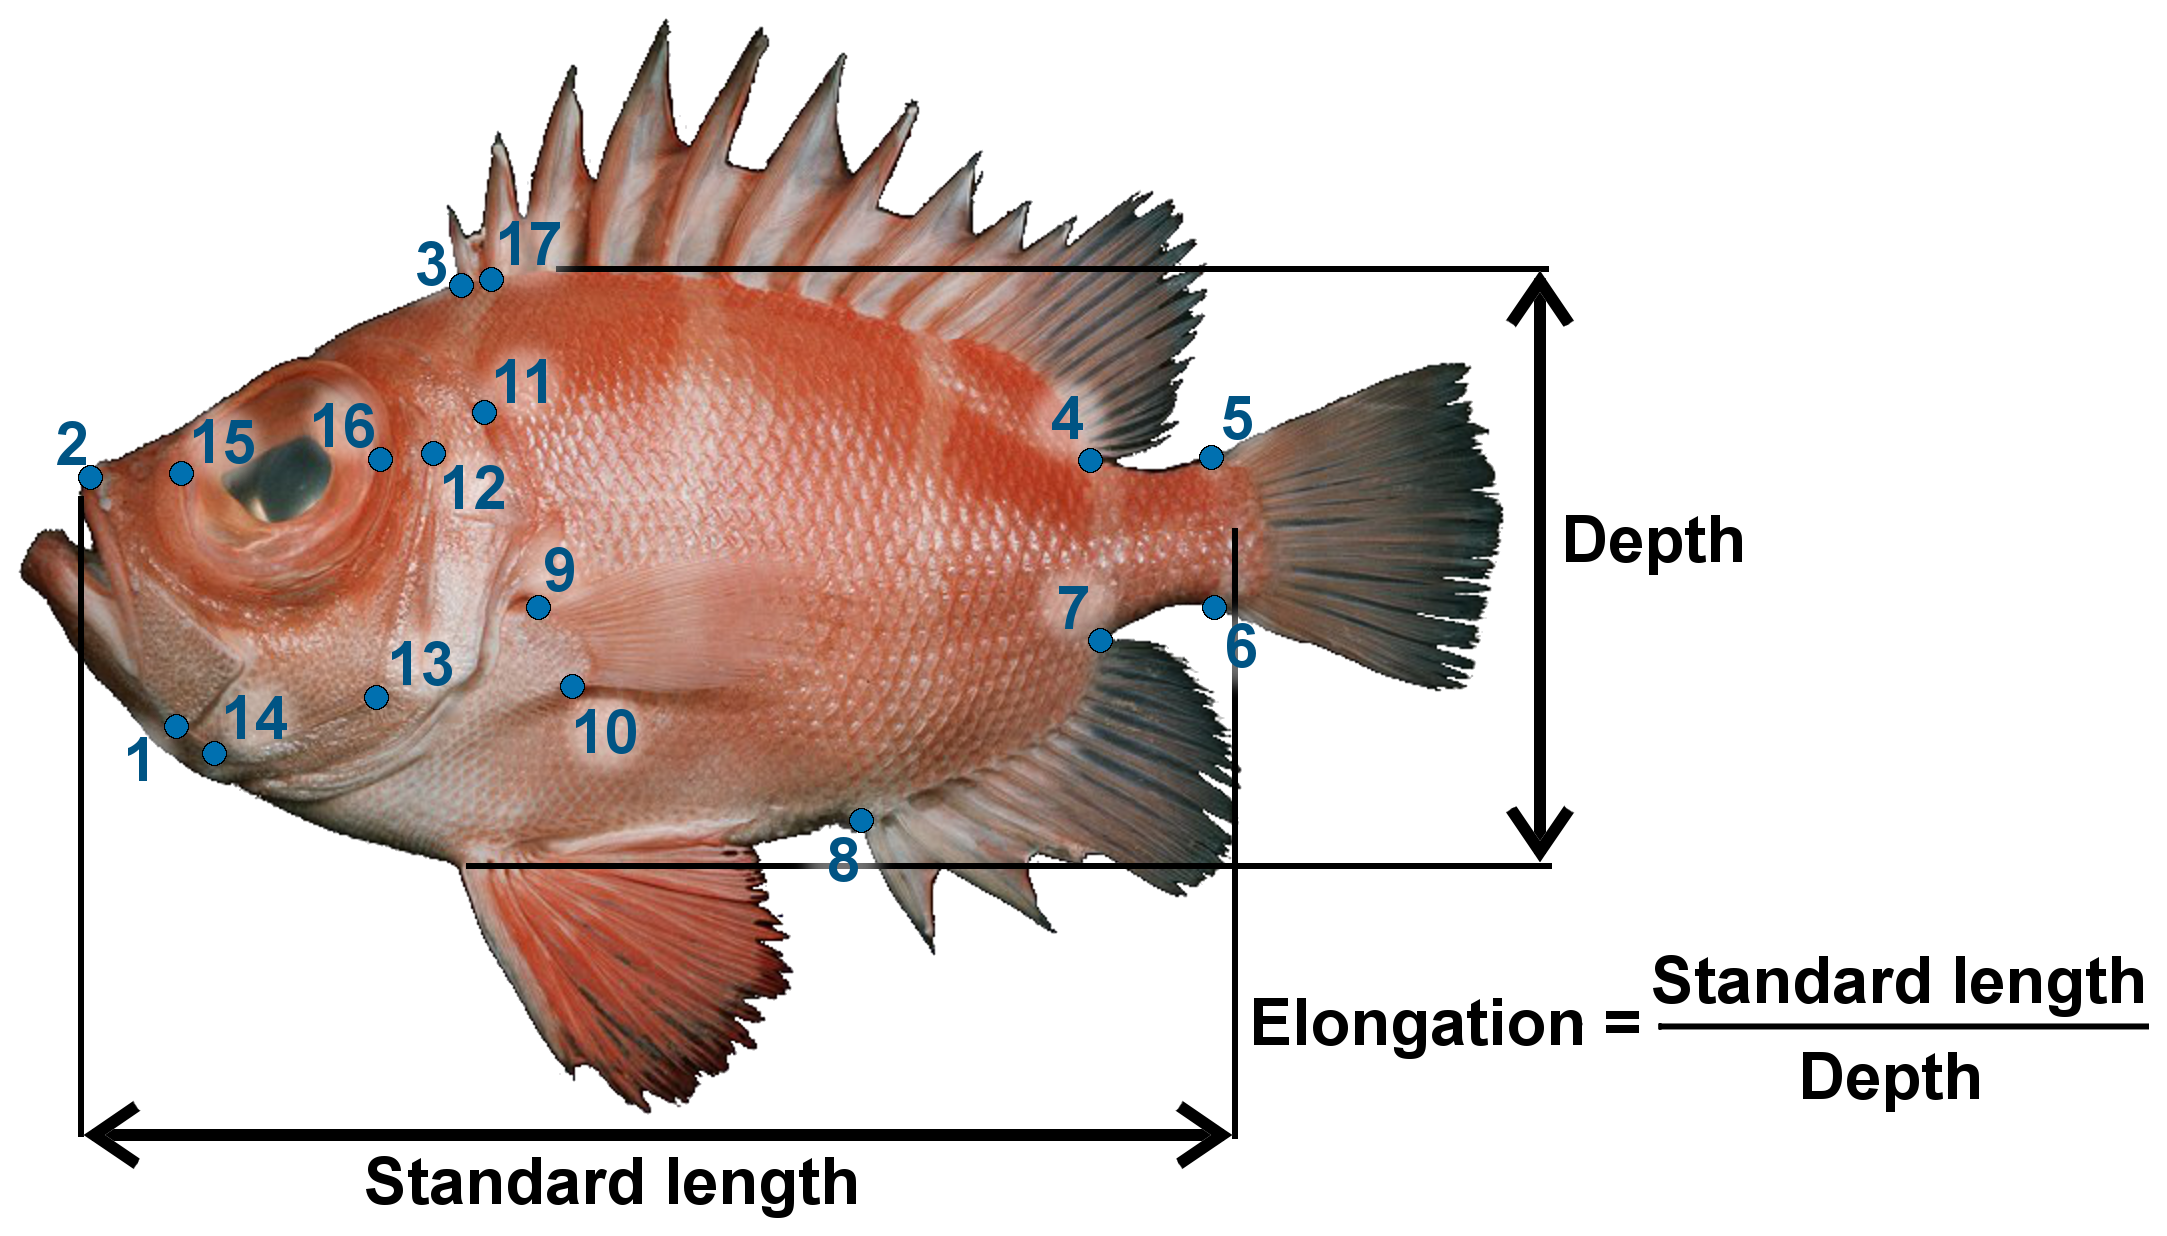
\includegraphics[height=\imageheight]{./media/EAWAG/pone.0112732.g001.png}%
		\sourcelink{https://doi.org/10.1371/journal.pone.0112732.g001}{DOI:gk6b4j}{Fig.~1}%
		}%
	\only<2>{%
		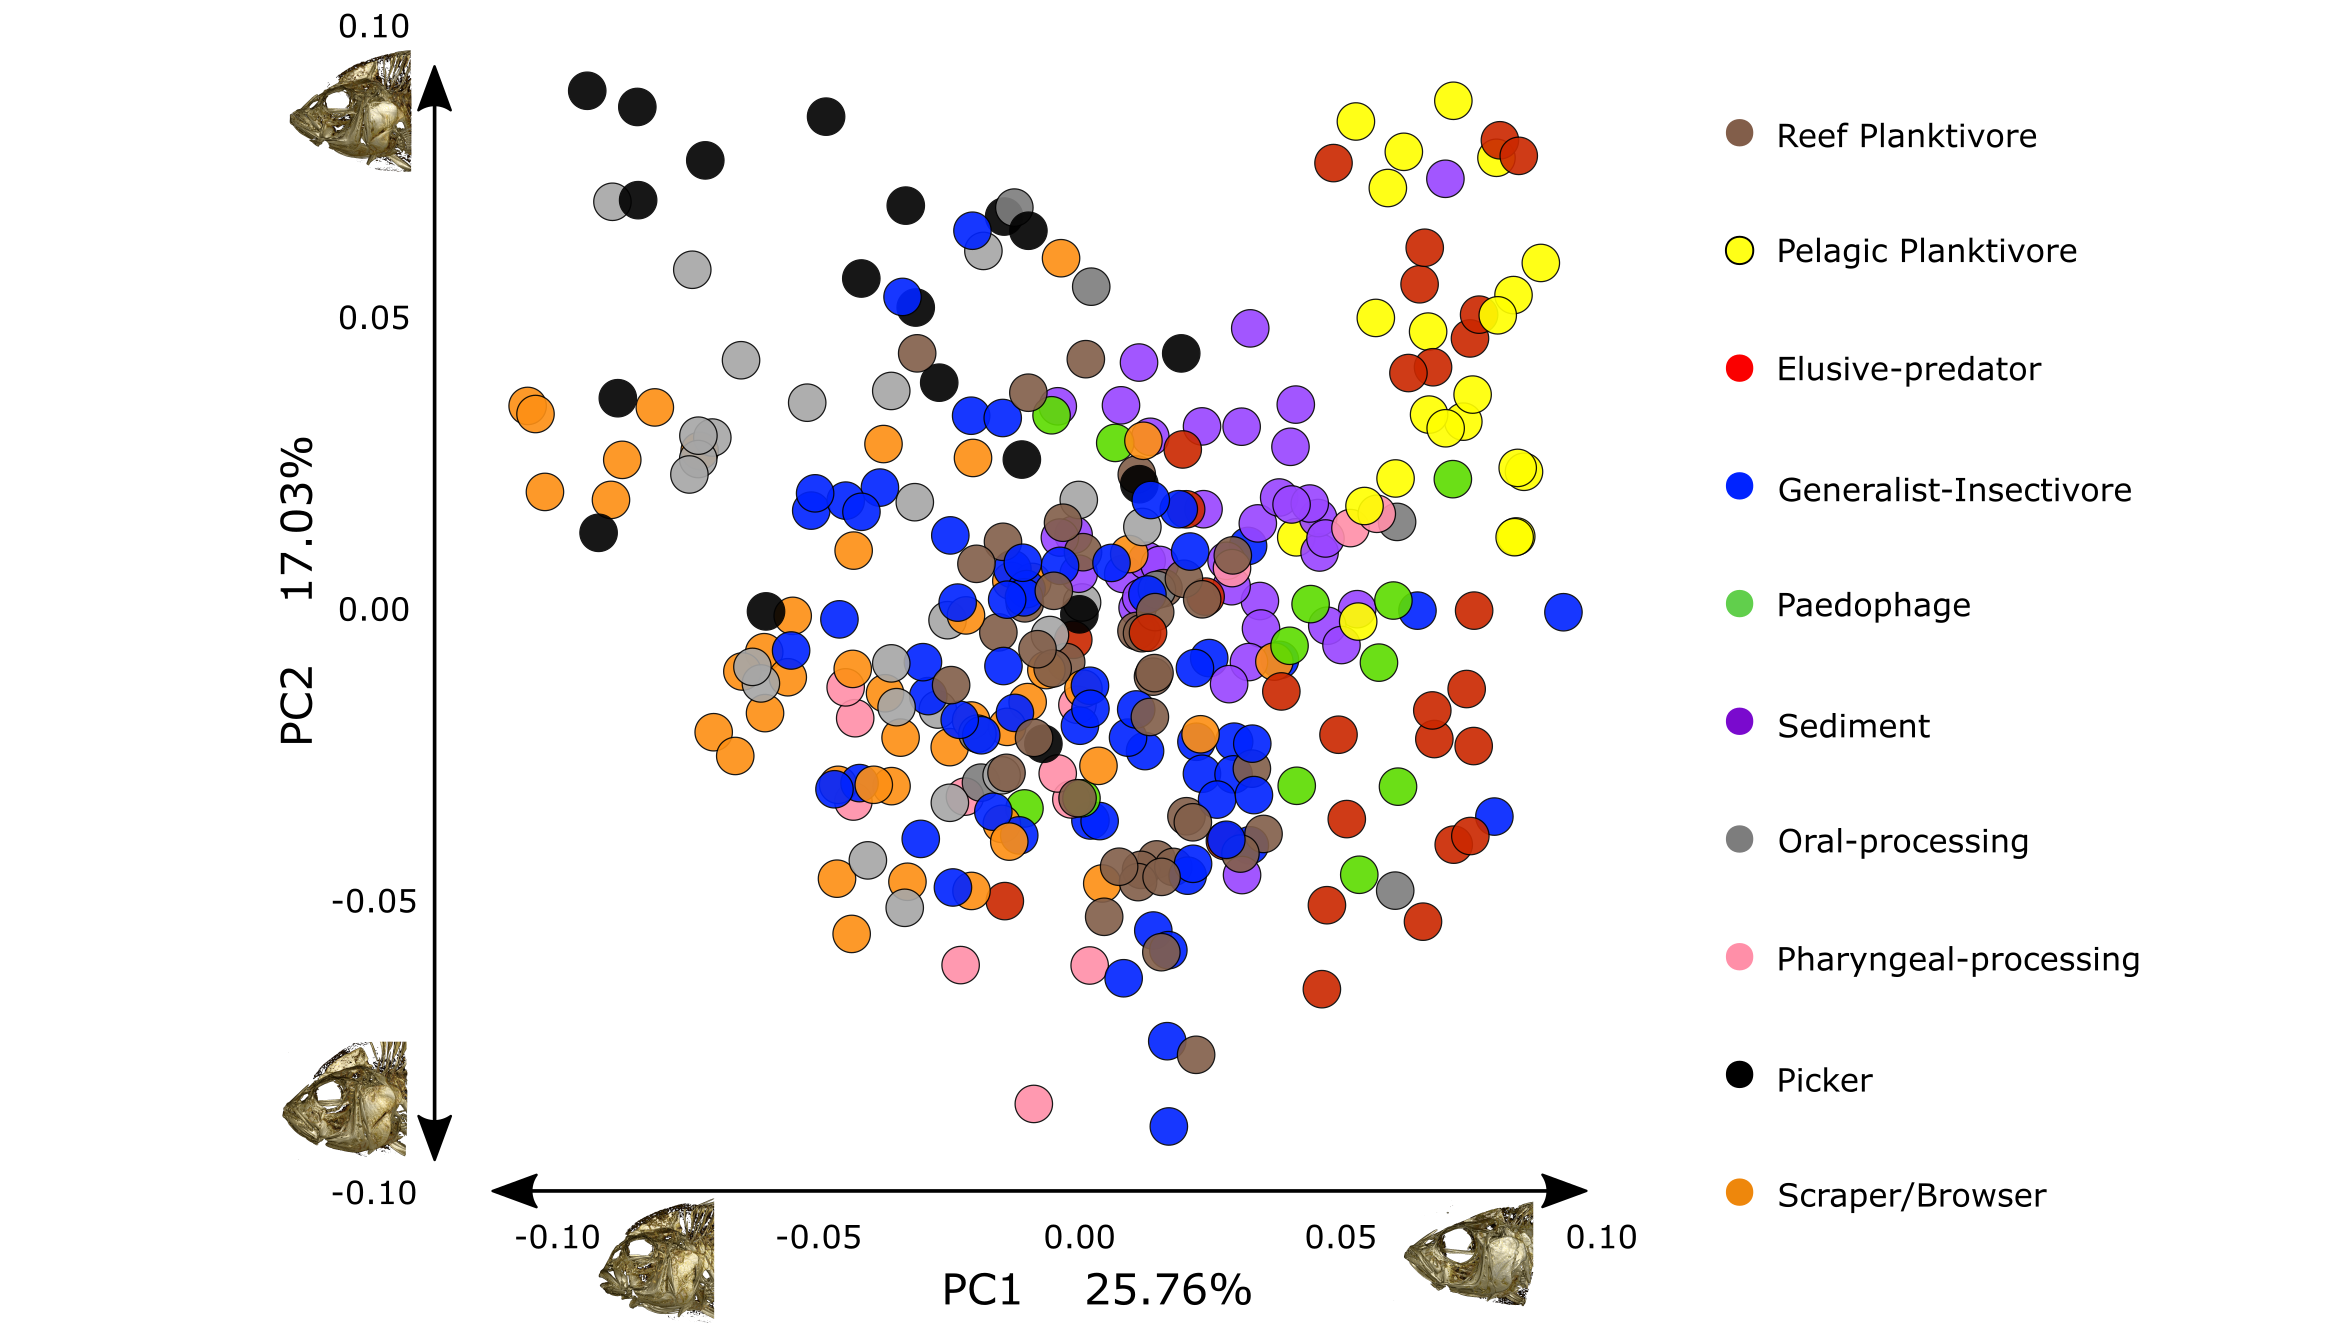
\includegraphics[height=\imageheight]{./media/EAWAG/3 PCA PC1vPC2 all specimens by diet}%
		\source{Kassandra Ford}{}%
		}%
	\note{Here are two figures; you are welcome to use either for an internal talk.
	One is a PCA with the individuals labeled by diet category, the other is a phylomorphospace, showing the same PCA but with additional phylogenetic data, again labeled by diet category.
	This is based on a 25-point landmark scheme on 1/2 of the head.}
\end{frame}

\begin{frame}
	\frametitle{More fish, but muscles}	
	\begin{columns}%
		\begin{column}{0.5\linewidth}%
			Collaboration with \emph{Developmental Biology and Regeneration} group of Nadia Mercader Huber~\footcite{Garcia-Poyatos2024}%
			\begin{itemize}%
				\item Influence of \emph{cox7a} on muscle volume%
				\item Confirmation of results by \uct%
				\item 2\(\times\)2\(\times\)5 Zebrafish, WT and KO%
			\end{itemize}%
		\end{column}%
		\begin{column}{0.5\linewidth}%
			\only<1>{%
				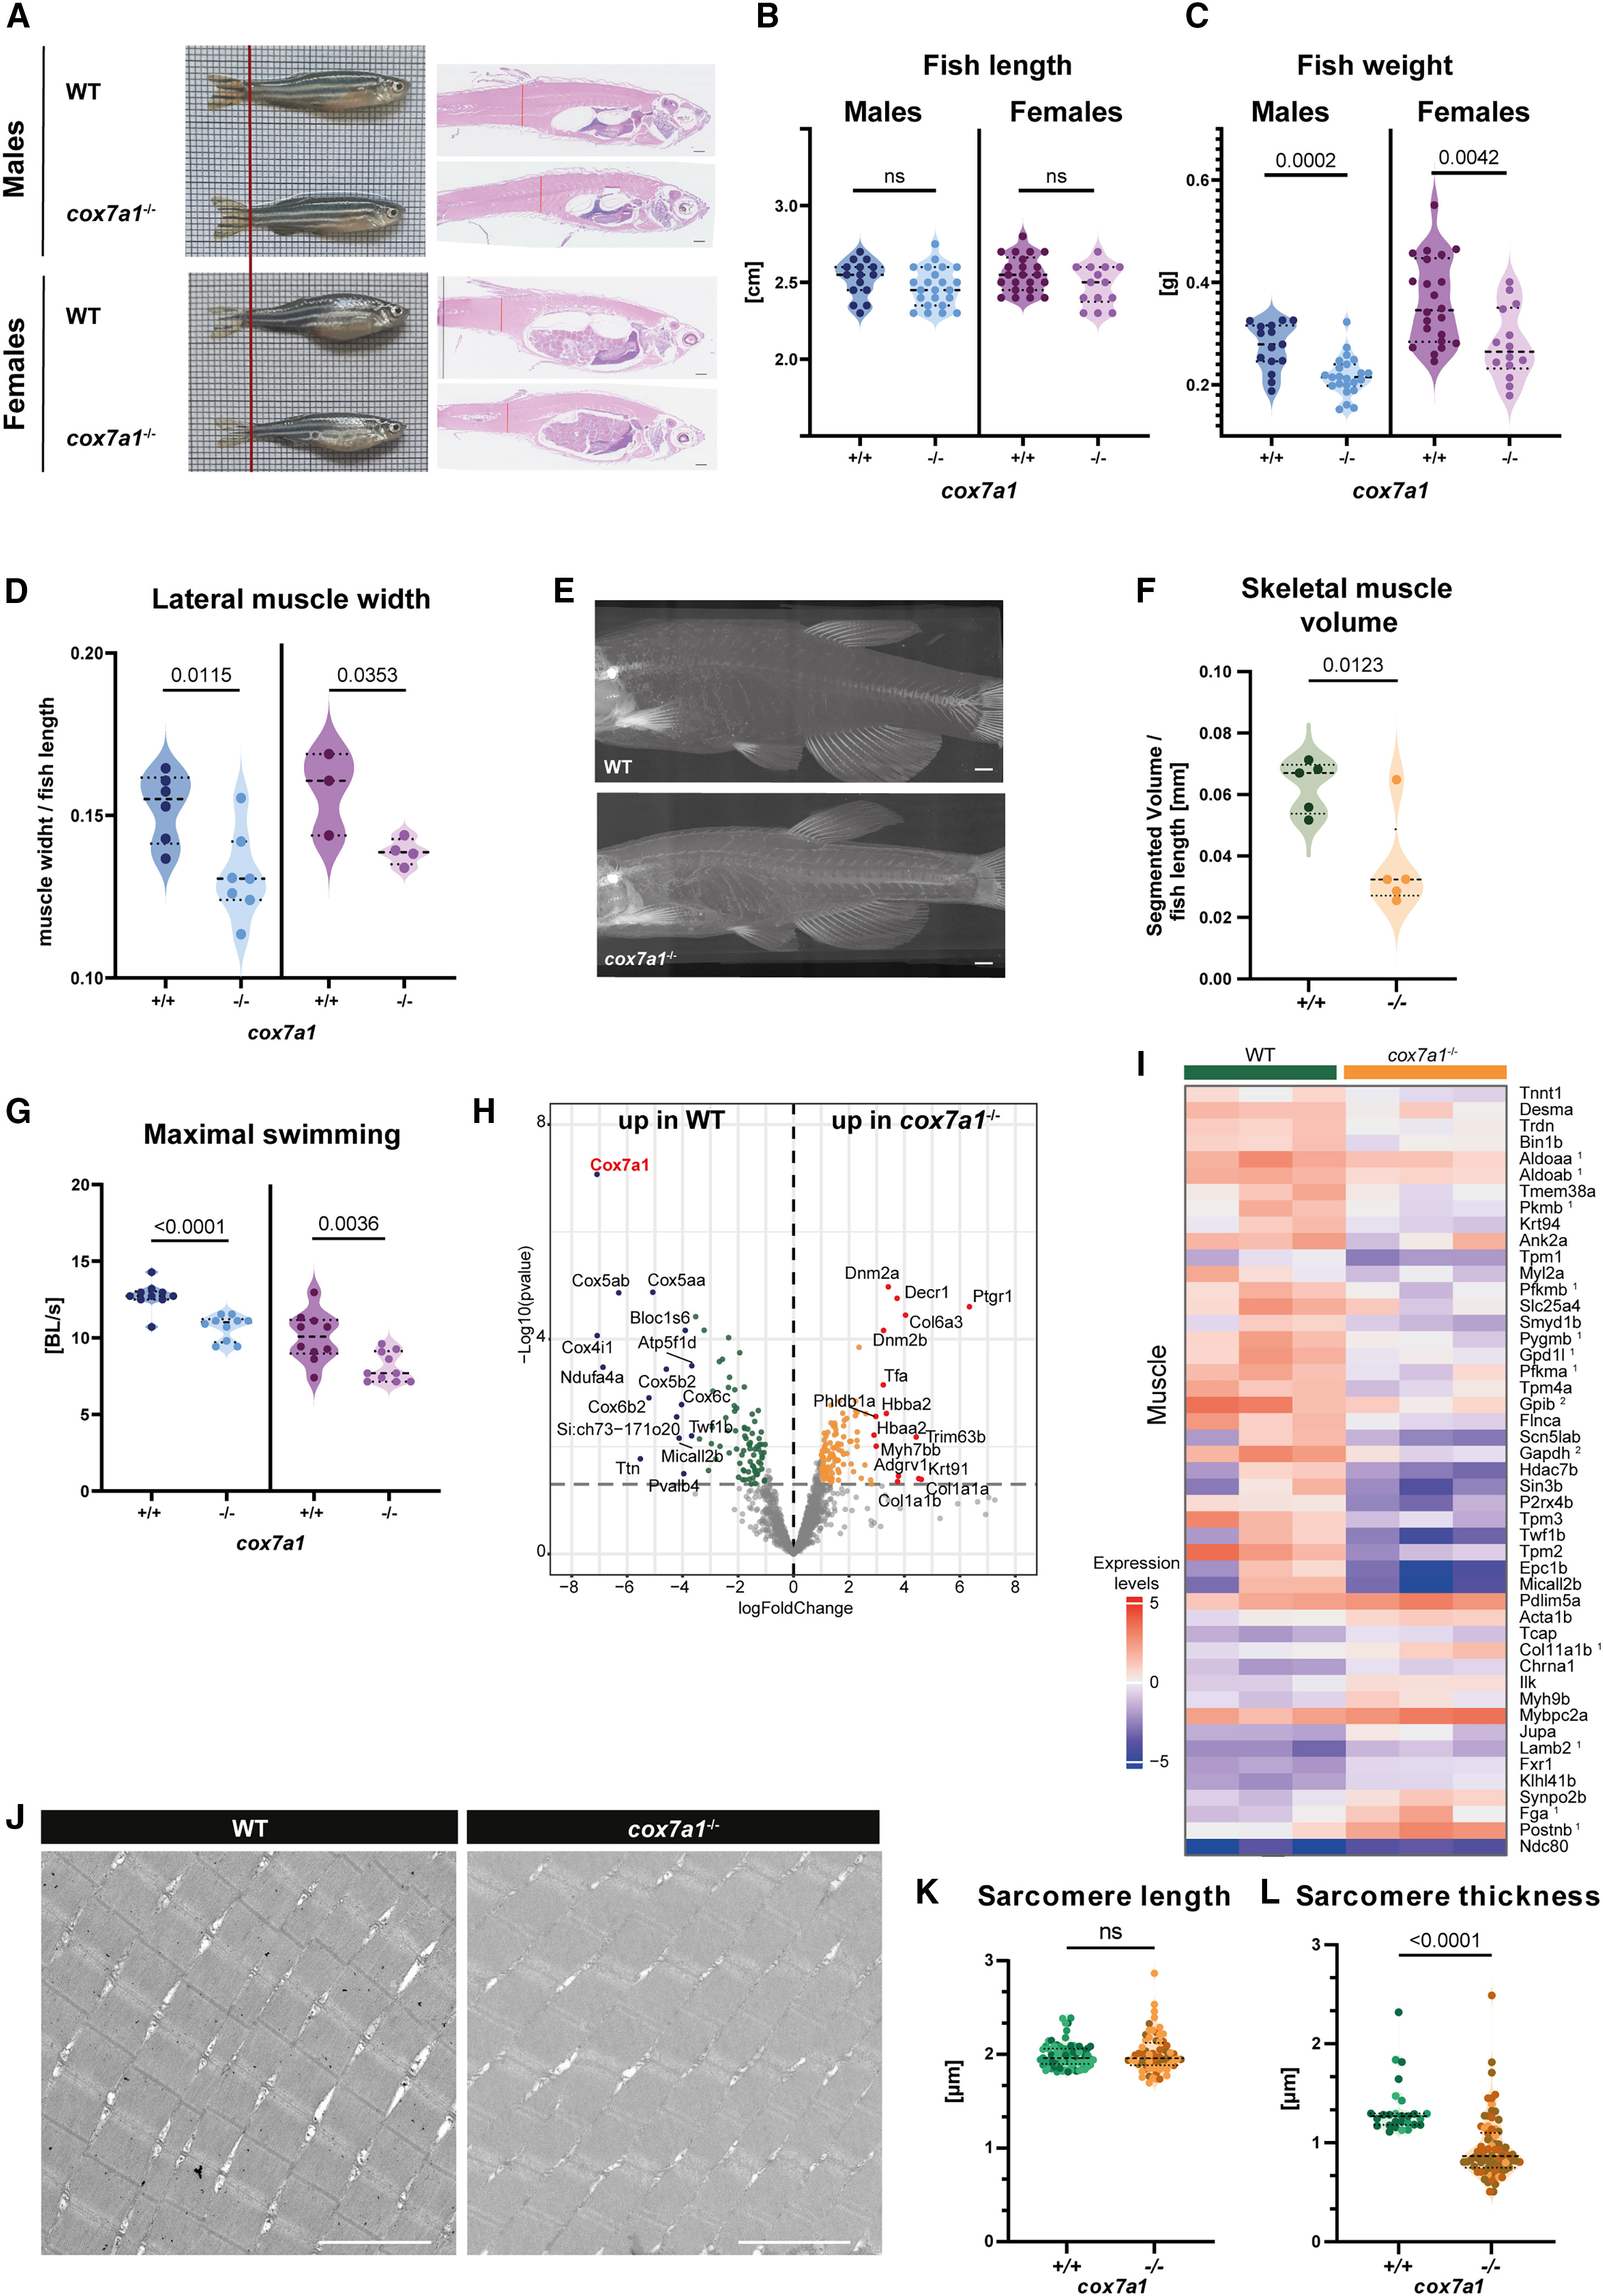
\includegraphics[height=\imageheight]{./media/cox7a/gr3_lrg}%
				\sourcelink{https://www.cell.com/developmental-cell/fulltext/S1534-5807(24)00237-5}{DOI:nh26}{Fig.~3}%
				}%
			\only<2>{%
				\lstinputlisting[linerange={2-4,15-15,17-19,28-30,36-37,40-40,45-45,53-54}]{./media/cox7a/5268A/proj/5268A.log}%
				}%
		\end{column}%
	\end{columns}%
\note{The oxidative phosphorylation (OXPHOS) system is dynamic and the respiratory complexes (RCs) coexist with super-assembled quaternary structures called supercomplexes (SCs). How assembly occurs and the physiological role of supercomplex assembly is still under intensive investigation. The Cox7a family member Cox7a2l, also known as Scaf1, promotes CIII-CIV super assembly and energetic efficiency in zebrafish, mice, and humans. Here we studied the role of a second member of the Cox7a family, Cox7a1 in SC assembly and striated muscle physiology. We found that this protein drives CIV homodimer formation, which increases CIV activity. The substantial reduction in CIV2 formation led to a profound metabolic rearrangement with a consequent non-pathological loss of skeletal muscle performance and muscle mass not observed in cox7a2l. Ablation of Cox7a1 also rewired heart metabolism. While overall cardiac function was not affected, the absence of Cox7a1, but not Cox7a2l increased cardiac regenerative capacity. In sum, we describe a high specificity of Cox7a isoform in controlling OXPHOS assembly and muscle metabolism. While overall OXPHOS activity is modified, the loss of CIII-CIV heterodimer formation or CIV homodimer formation have very distinct metabolic and physiological consequences, highlighting the complexity of OXPHOS function and the importance of cox7a1 in striated muscle maturation.}
\end{frame}

\begin{frame}
	\frametitle{Volumetry}
		\begin{columns}
		  \begin{column}{0.5\linewidth}
			  \begin{itemize}
					\item<1-> Cutting samples to consistent (\(\neq\) equal!) length
					\item<2-> Gray value histogram shows difference
					\item<4-> Simple thresholding and volume counting
					\item<5-> Segmentation
					\item<6-> \blockquote[Carla Lembke][]{The mutant was 5269, the wildtype was 5268. [...], all males.}
			  \end{itemize}
		  \end{column}
		  \begin{column}{0.5\linewidth}
			  \centering
			  \includegraphics<1>[width=\imagewidth]{./media/cox7a/cut.5268C.png}\\%
			  \includegraphics<1>[width=\imagewidth]{./media/cox7a/cut.5269C.png}%
			  \includegraphics<2>[width=\imagewidth]{./media/cox7a/grayvaluehistogram.png}%
			  \includegraphics<3>[width=\imagewidth]{./media/cox7a/grayvaluehistogram.log.png}%
			  \includegraphics<4>[width=\imagewidth]{./media/cox7a/Volume_Boxplot.5268_5269.ThresholdedVolumeLargestComponent.png}%
			  \includegraphics<5>[width=0.5\imagewidth]{./media/cox7a/histogram.5268C.png}%
			  \includegraphics<5>[width=0.5\imagewidth]{./media/cox7a/histogram.5269C.png}%
			  \includegraphics<6>[width=\imagewidth]{./media/cox7a/Volume_Boxplot.5268_5269.SegmentedVolumemm3}%
		  \end{column}
	  \end{columns}
  \end{frame}

\begin{frame}
	\frametitle{Adiöwou}
	\begin{itemize}
		\item \uct provides insights into samples not otherwise possible
		\item Unbiased segmentation
		\item Simple algorithms can lead to nice data
		\item Ask anything!
	\end{itemize}
\end{frame}

\begin{frame}[allowframebreaks]
	\frametitle{References}
	\renewcommand*{\bibfont}{\small}
	%\setbeamertemplate{bibliography item}{\insertbiblabel}
	\printbibliography{}
\end{frame}

\end{document}